\documentclass[11pt]{article}
\usepackage[margin=1.02in]{geometry}
\usepackage{amsmath,amssymb,amsthm,mathtools}
\usepackage{graphicx}
\usepackage{xcolor}
\usepackage[hidelinks]{hyperref}
\usepackage{microtype}

\newtheorem{theorem}{Theorem}
\newtheorem{lemma}{Lemma}
\newcommand{\R}{\mathbb R}
\newcommand{\Ext}{\operatorname{Ext}}
\newcommand{\conv}{\operatorname{conv}}
\newcommand{\JB}{\perp_{B}}
\newcommand{\JBe}[1]{\perp_{B}^{#1}}

\definecolor{statusred}{RGB}{156,36,31}

\title{A Two-Dimensional Counterexample to\\
Finite-Dimensional C-Approximate Symmetry}
\author{fa\_banach\_001 / agent\_lane\_00}
\date{19 July 2026}

\begin{document}
\maketitle

\noindent
\fcolorbox{statusred}{statusred!6}{%
  \begin{minipage}{0.92\textwidth}
  \textbf{Status: candidate counterexample, likely valid.}
  The constructed two-dimensional norm has local property (P) at every
  sphere point, but its Birkhoff--James orthogonality is not globally
  C-approximately symmetric.  This disproves Conjecture~3.11 of the source.
  \end{minipage}}

\section{Source conjecture}

Chmieli\'nski, Khurana, and Sain formulate the following on PDF page~16 of
\emph{Local approximate symmetry of Birkhoff--James orthogonality in normed
linear spaces}, arXiv:2012.08162 \cite{CKS}:

\begin{quote}
Let $X$ be a finite-dimensional Banach space. Then the Birkhoff--James
orthogonality is C-approximately symmetric in $X$ if and only if the local
property (P) holds for each $x\in\Ext B_X$.
\end{quote}

\begin{figure}[ht]
  \centering
  
\includegraphics[width=\textwidth]{figures/open_problem_crop.png}
  \caption{Conjecture~3.11 as rendered from page~16 of the source paper.}
\end{figure}

\section{Definitions}

For $x\in S_X$, let
\[
 J(x)=\{f\in S_{X^*}:f(x)=1\}.
\]
The support-functional characterizations used in the source are
\begin{align*}
 x\JB y &\quad\Longleftrightarrow\quad
     \text{some }f\in J(x)\text{ satisfies }f(y)=0,\\
 x\JBe{\varepsilon}y &\quad\Longleftrightarrow\quad
     \text{some }f\in J(x)\text{ satisfies }
     |f(y)|\leq\varepsilon\lVert y\rVert.
\end{align*}
The relation is globally C-approximately symmetric if one
$\varepsilon<1$ works in
\[
 x\JB y\quad\Longrightarrow\quad y\JBe{\varepsilon}x
\]
for all $x,y$.

The local property (P) holds at $x\in S_X$ when there is no
$y\in S_X$ such that $x\JB y$ and every $f\in J(y)$ belongs, up to
sign, to $J(x)$.  Equivalently, whenever $x\JB y$, at least one
$f\in J(y)$ lies outside $J(x)\cup(-J(x))$.

\section{Proof intuition}

Pointwise property (P) only asks for a strict reverse support gap for each
orthogonal pair; it does not say that these gaps stay uniformly away from
one.  The construction makes this distinction visible.  Its unit sphere has
a flat top facet and a smooth curved arc approaching the left endpoint of
that facet.  Tangents to the arc are parallel to points moving toward the
right endpoint of the facet.  This gives exact orthogonal pairs whose reverse
support evaluations approach one.

At the limiting corners, extra supporting functionals appear.  Those extra
supports ensure property (P) at the limit, even though they cannot prevent
the pre-limit reverse constants from tending to one.  The norm is therefore
nonpolyhedral and nonsmooth exactly where the compactness argument behind the
conjecture loses upper semicontinuity.

\section{The counterexample}

Define $u:[-1,1]\to\R$ by
\[
 u(t)=
 \begin{cases}
  -1+2\sqrt{1+t},&-1\leq t\leq0,\\
  1,&0\leq t\leq1,
 \end{cases}
\]
and set
\begin{equation}
 K=\{(s,t)\in\R^2:-1\leq s\leq1,\ -u(-s)\leq t\leq u(s)\}.
 \label{eq:K}
\end{equation}
Let $X$ be $\R^2$ with unit ball $K$.

\begin{figure}[ht]
  \centering
  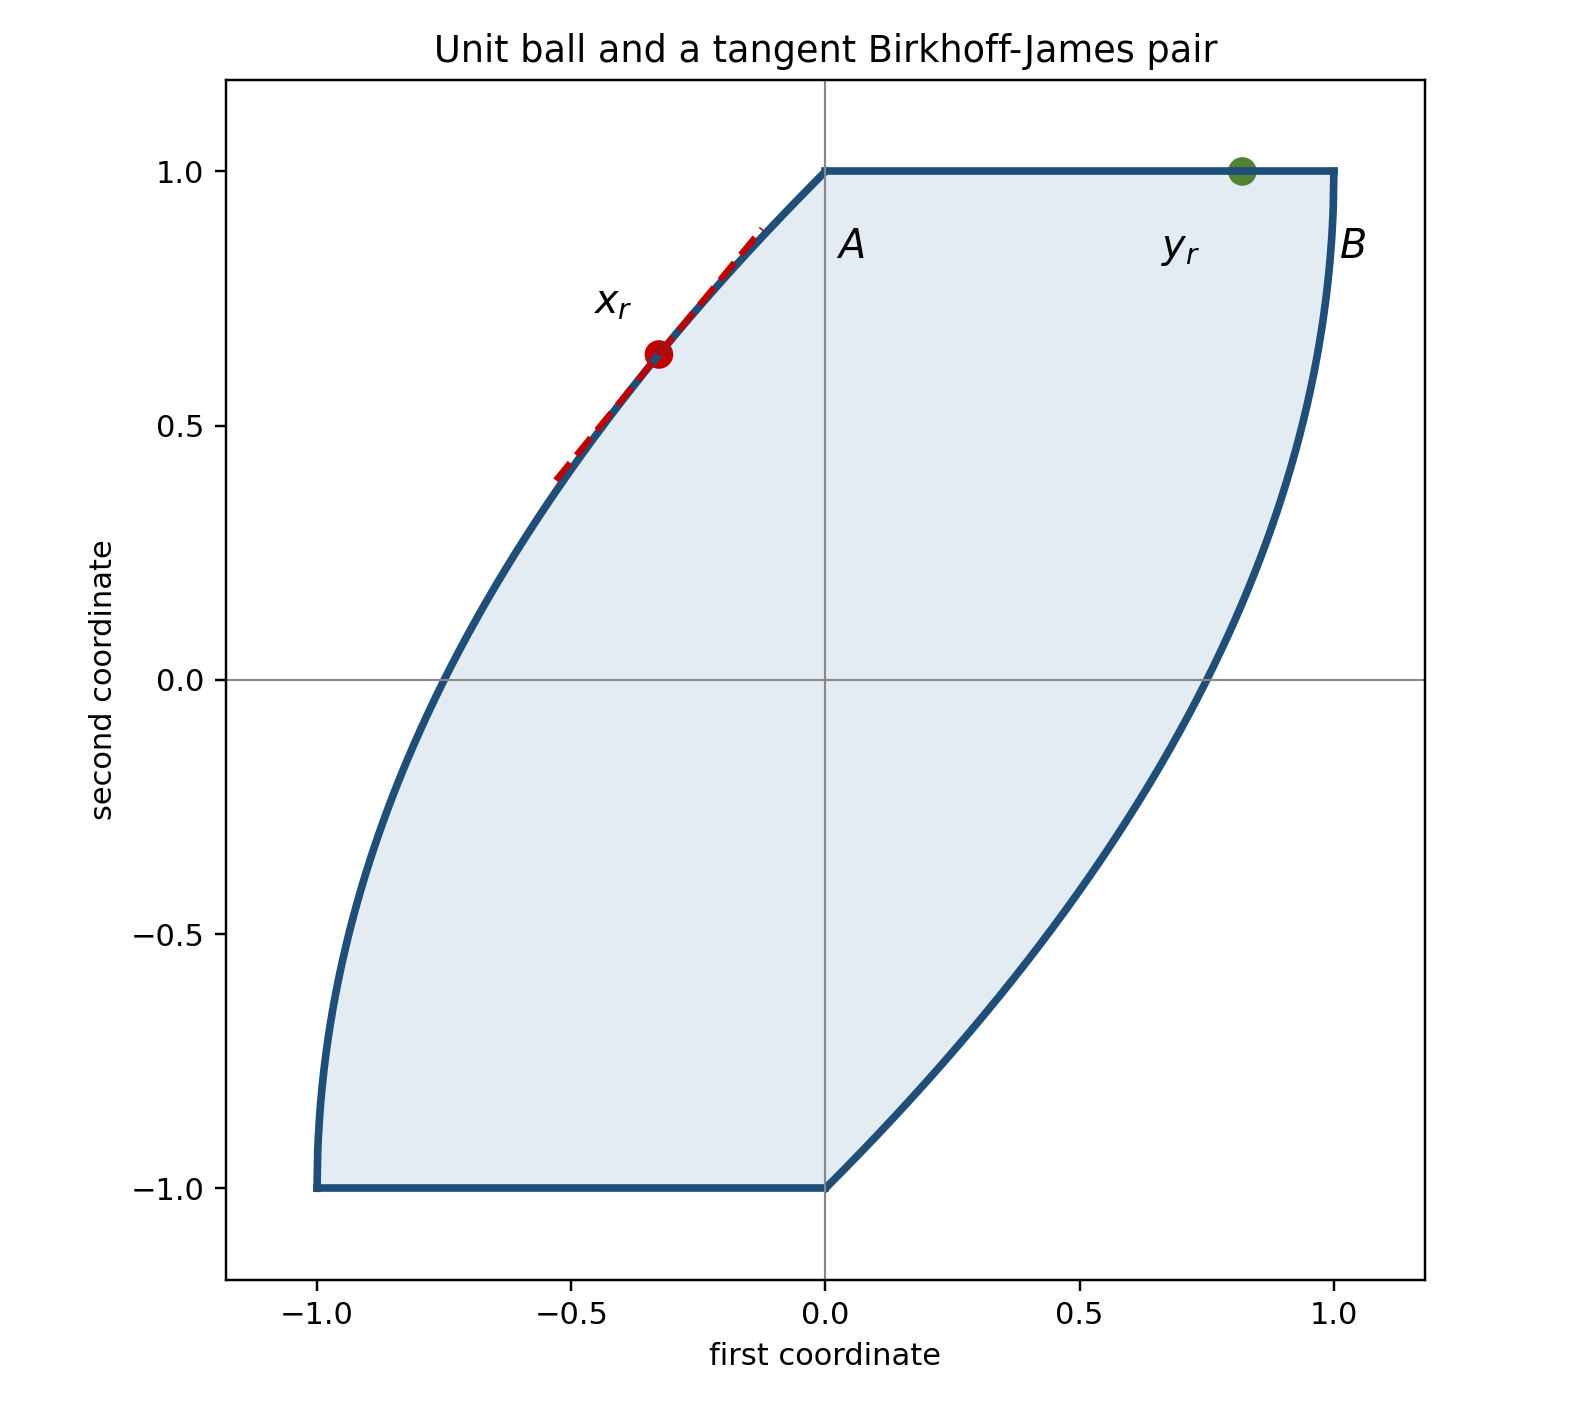
\includegraphics[width=0.78\textwidth]{figures/unit_ball_geometry.png}
  \caption{The unit ball.  The dashed tangent at $x_r$ is parallel to
  $y_r$, while $y_r$ lies in the relative interior of the top facet.}
\end{figure}

\begin{theorem}
\label{thm:counterexample}
The two-dimensional Banach space $X$ defined by \eqref{eq:K} has local
property (P) at every point of $S_X$.  Nevertheless, Birkhoff--James
orthogonality in $X$ is not globally C-approximately symmetric.
Consequently, $X$ is a counterexample to Conjecture~3.11.
\end{theorem}

\begin{proof}
\textbf{Step 1: $K$ is a unit ball.}
On $(-1,0)$,
\[
 u'(s)=\frac{1}{\sqrt{1+s}},\qquad
 u''(s)=-\frac{1}{2(1+s)^{3/2}}<0.
\]
At zero the one-sided slope drops from $1$ to $0$.  Hence $u$ is concave.
The lower boundary $-u(-s)$ is convex, so $K$ is convex.  It is compact,
centrally symmetric, and contains the origin in its interior.  It is
therefore the closed unit ball of a norm on $\R^2$.

The boundary is smooth except at
\[
 A=(0,1),\qquad B=(1,1),\qquad -A,\qquad -B.
\]
Every smooth sphere point has local property (P), as observed in the source.
It remains to check these four corners.  Central symmetry reduces this to
$A$ and $B$.

\textbf{Step 2: property (P) at $A$.}
Write the functionals as coordinate pairs.  The top facet and the tangent to
the square-root arc at $A$ give
\[
 g=(0,1),\qquad h=(-1,1),\qquad
 J(A)=\conv\{g,h\}=\{(-s,1):0\leq s\leq1\}.
\]
Suppose $A\JB z$.  Up to replacing $z$ by $-z$, some positive multiple of
$z$ lies on a ray
\[
 t=sx,\qquad 0\leq s\leq1,quad x>0.
\]
For $s<1$, this ray meets the relative interior of the smooth right-hand arc
\[
 \Gamma_R=\{(x,1-2\sqrt{1-x}):0<x<1\}.
\]
Indeed, its defining function has derivative
$1/\sqrt{1-x}>1\geq s$, begins below the ray, and ends above it.  The
intersection is unique.  The unique supporting functional there cannot lie
in $J(A)\cup(-J(A))$: the functionals in $J(A)$ expose either $A$ alone or
the top facet $[A,B]$, and their negatives expose the opposite faces.

For $s=1$, the ray meets $B$.  But $k=(1,0)$ belongs to $J(B)$ and lies
outside $J(A)\cup(-J(A))$.  Thus every $z$ with $A\JB z$ has a support
outside the signed support set of $A$, proving property (P) at $A$.

\textbf{Step 3: property (P) at $B$.}
The top facet and the vertical tangent at $B$ give
\[
 J(B)=\conv\{g,k\}=\{(s,1-s):0\leq s\leq1\}.
\]
For $s<1$, a kernel line of $(s,1-s)$ has, in the right half-plane,
slope $-s/(1-s)$.  It meets $\Gamma_R$ at a unique smooth point.  As before,
the unique support there lies outside $J(B)\cup(-J(B))$, since functionals
in $J(B)$ expose only $B$ or the top facet, and the negative functionals
expose their opposites.  For $s=1$, the kernel is the vertical axis and meets
$S_X$ at $\pm A$; the functional $h\in J(A)$ (or its negative) lies outside
$J(B)\cup(-J(B))$.  Hence property (P) holds at $B$, and therefore at all
four corners.  We have proved property (P) on all of $S_X$, stronger than
the extreme-point hypothesis in the conjecture.

\textbf{Step 4: no uniform reverse constant.}
For $1/2<r<1$, define
\[
 x_r=(r^2-1,2r-1),\qquad y_r=(r,1).
\]
Since
\[
 u(r^2-1)=-1+2\sqrt{r^2}=2r-1,
\]
$x_r$ belongs to the smooth square-root arc, while $y_r$ belongs to the
relative interior of the top facet.  The slope of the arc at $x_r$ is $1/r$,
so its tangent vector $(1,1/r)$ is parallel to $y_r=(r,1)$.  The supporting
functional at $x_r$ annihilates $y_r$, and hence
\[
 x_r\JB y_r.
\]

The unique element of $J(y_r)$ is $g=(0,1)$.  By the approximate
orthogonality characterization,
\[
 y_r\JBe{\varepsilon}x_r
 \quad\Longleftrightarrow\quad
 |g(x_r)|=2r-1\leq\varepsilon.
\]
Thus the least reverse constant for this pair is $2r-1$, which tends to one
as $r\uparrow1$.  Given any $\varepsilon<1$, choosing
$r>(1+\varepsilon)/2$ gives $x_r\JB y_r$ but
$y_r\not\JBe{\varepsilon}x_r$.  No global C-approximate symmetry constant
exists.
\end{proof}

\section{Verification}

The script \texttt{code/verify\_geometry.py} samples the full boundary,
checks the named supporting functionals, verifies five tangent pairs, and
stress-tests 2,000 kernel directions at each positive corner.  It reports
exact named supports, tangent residual $1.11\times10^{-16}$, and no sampled
support entering either forbidden signed corner segment.  The largest sampled
reverse constant is $0.9998$.  Full commands and residuals appear in
\texttt{verification.md}; the computation is not used as proof.

\section{Scope and bounded novelty check}

The result disproves the finite-dimensional equivalence exactly as stated; it
does not affect the source's theorems for polyhedral or smooth spaces.  The
counterexample is necessarily outside both classes: it has flat facets,
curved arcs, and four nonsmooth junctions.

The run's cheap indexes were searched by arXiv id, title, and the phrases
``C-approximately symmetric'', ``local property (P)'', and
``Birkhoff--James''.  A bounded web/arXiv search used the exact conjecture
language and author/title combinations.  It found the source and nearby
local-symmetry work, but no later resolution or matching construction.  This
is a bounded check, not an exhaustive novelty claim.

\section{Human-review recommendation}

This packet is suitable for mathematical review.  The highest-value checks
are the endpoint cases in Steps 2--3 and the use of the unique top-facet
support in Step~4.  Until review, retain the status
\emph{candidate counterexample, likely valid}.

\section{Reference}

\begin{thebibliography}{9}
\bibitem{CKS}
J. Chmieli\'nski, D. Khurana, and D. Sain,
\emph{Local approximate symmetry of Birkhoff--James orthogonality in normed
linear spaces}, Results Math. \textbf{76} (2021), Article 136;
arXiv:2012.08162.
\end{thebibliography}

\end{document}
